\documentclass[a4paper, 10pt]{article} % Tamanho de fonte menor

\setlength{\headheight}{34.54448pt}
\addtolength{\topmargin}{-32.54448pt} % Ajustei mais a margem superior
\setlength{\headsep}{10pt} % Aumento do espaçamento entre a borda superior e o cabeçalho

\usepackage[portuguese]{babel}
\usepackage[utf8]{inputenc}
\usepackage{amsmath}
\usepackage{amssymb}
\usepackage{graphicx}
\usepackage{float}
\usepackage{subcaption}
\usepackage{color}
\usepackage{indentfirst}
\setlength{\marginparwidth}{2cm}
\usepackage{fancyhdr} % Pacote para cabeçalho
\usepackage{verbatim}
\usepackage{textcomp}
\usepackage{gensymb}
\usepackage{geometry}
\usepackage{listings}
\usepackage{xcolor}
\usepackage{hyperref}

% Ajuste das margens
\geometry{
    top=0.9in, % Margem superior ajustada para 0.9 polegadas
    bottom=1.in, % Margem inferior
    left=1.1in, % Margem esquerda
    right=1in, % Margem direita reduzida
}
\begin{document}

\begin{titlepage}
	\begin{center}
		\begin{figure}[htb!]
			\begin{center}
				
\includegraphics[width=3.9cm]{Logo_UnB.png}
			\end{center}
		\end{figure}
        \Large{\textbf{Universidade de Brasília}}\\
        \Large{FCTE}\\
        \Large{Instrumentação Eletrônica}\\

        \vspace{100pt}

        \LARGE{\textbf{Instrumentação Eletrônica: Trabalho Final}}\\

        \vspace{120pt}


        \vspace{20pt}
        \hfill  Felipe de Castro Quixabeira \hspace{20pt} Mat: 231026812  \\
        \hfill  Gabriel Celestino de Almeida \hspace{20pt} Mat: 231027079  \\

        \vspace{25pt}
        \hfill \underline{Professor:}\\
        \hfill Claudia Ochoa\\ %Entre com o nome do professor


        \vfill
        \begin{center}
        Brasília

        2026

        \thispagestyle{empty}
    \end{center}
	\end{center}
\end{titlepage}

\newpage

% Configuração do cabeçalho
\pagestyle{fancy}
\fancyhf{}
\fancyhead[L]{Universidade de Brasília \\ Faculdade de Ciências e Tecnologias em Engenharia \\ Engenharia Eletrônica}
\fancyhead[R]{
\includegraphics[width=1.5cm]{Logo_UnB.png}}

\tableofcontents
\newpage
%Escrever aqui

\section{Introdução}
Sensores acelerômetros são utilizados em múltiplas aplicações, atualmente encontramos eles em aplicações de robótica, interações de controle gestual, controle de veículos aéreos não tripulados e diversos outros usos.
Para utilizarmos de forma apropriada os sensores desse tipo é necessário compreender os princípios físicos por trás do funcionamento de diferentes tipos de acelerômetros, como se originam suas principais fontes de erro, as principais características das leituras realizadas e as formas adequadas de obtenção dos dados.

\section{Objetivos}
O objetivo do trabalho proposto é estudar o funcionamento do sensor acelerômetro da Unidade de Medição Inercial MPU 6050, extrair as suas principais características a partir da folha de dados (\textit{datasheet}) e verificar o funcionamento do sensor experimentalmente.

\section{Fundamentação Teórica}

\subsection{Acelerômetro}
O acelerômetro é um transdutor capaz de medir aceleração, ele é responsável por converter grandeza mecânica em sinais elétricos. Dentre os acelerômetros que existem os que se destacam são os baseados em MEMS (\textit{Micro-Electro-Mechanical Systems}), que utilizam elementos mecânicos muito pequenos, de escala micrométrica, ocasionando no baixo consumo energético e custo.

\subsection{Princípio de Funcionamento}
Internamente o sistema pode ser interpretado como uma pequena massa suspensa por molas microscópicas, onde preso nessa massa existem várias ``linhas" de silício similares aos dentes de um pente entrelaçam-se com outros dentes fixos no chip (Figura~\ref{fig:mems}). Quando se move o sensor, a massa se desloca e muda a distância e consequentemente a capacitância entre as peças é alterada, tendo como resultado uma variação elétrica, que permite calcular quanto de força se aplicou em um dos eixos \cite[pp.~224--226]{aguirre2013fundamentos}. Existe no chip circuitos de condicionamento que convertem essa variação em um valor digital de 16 bits.

\begin{figure}[H]
	\centering
	\begin{subfigure}[b]{0.55\textwidth}
		\centering
		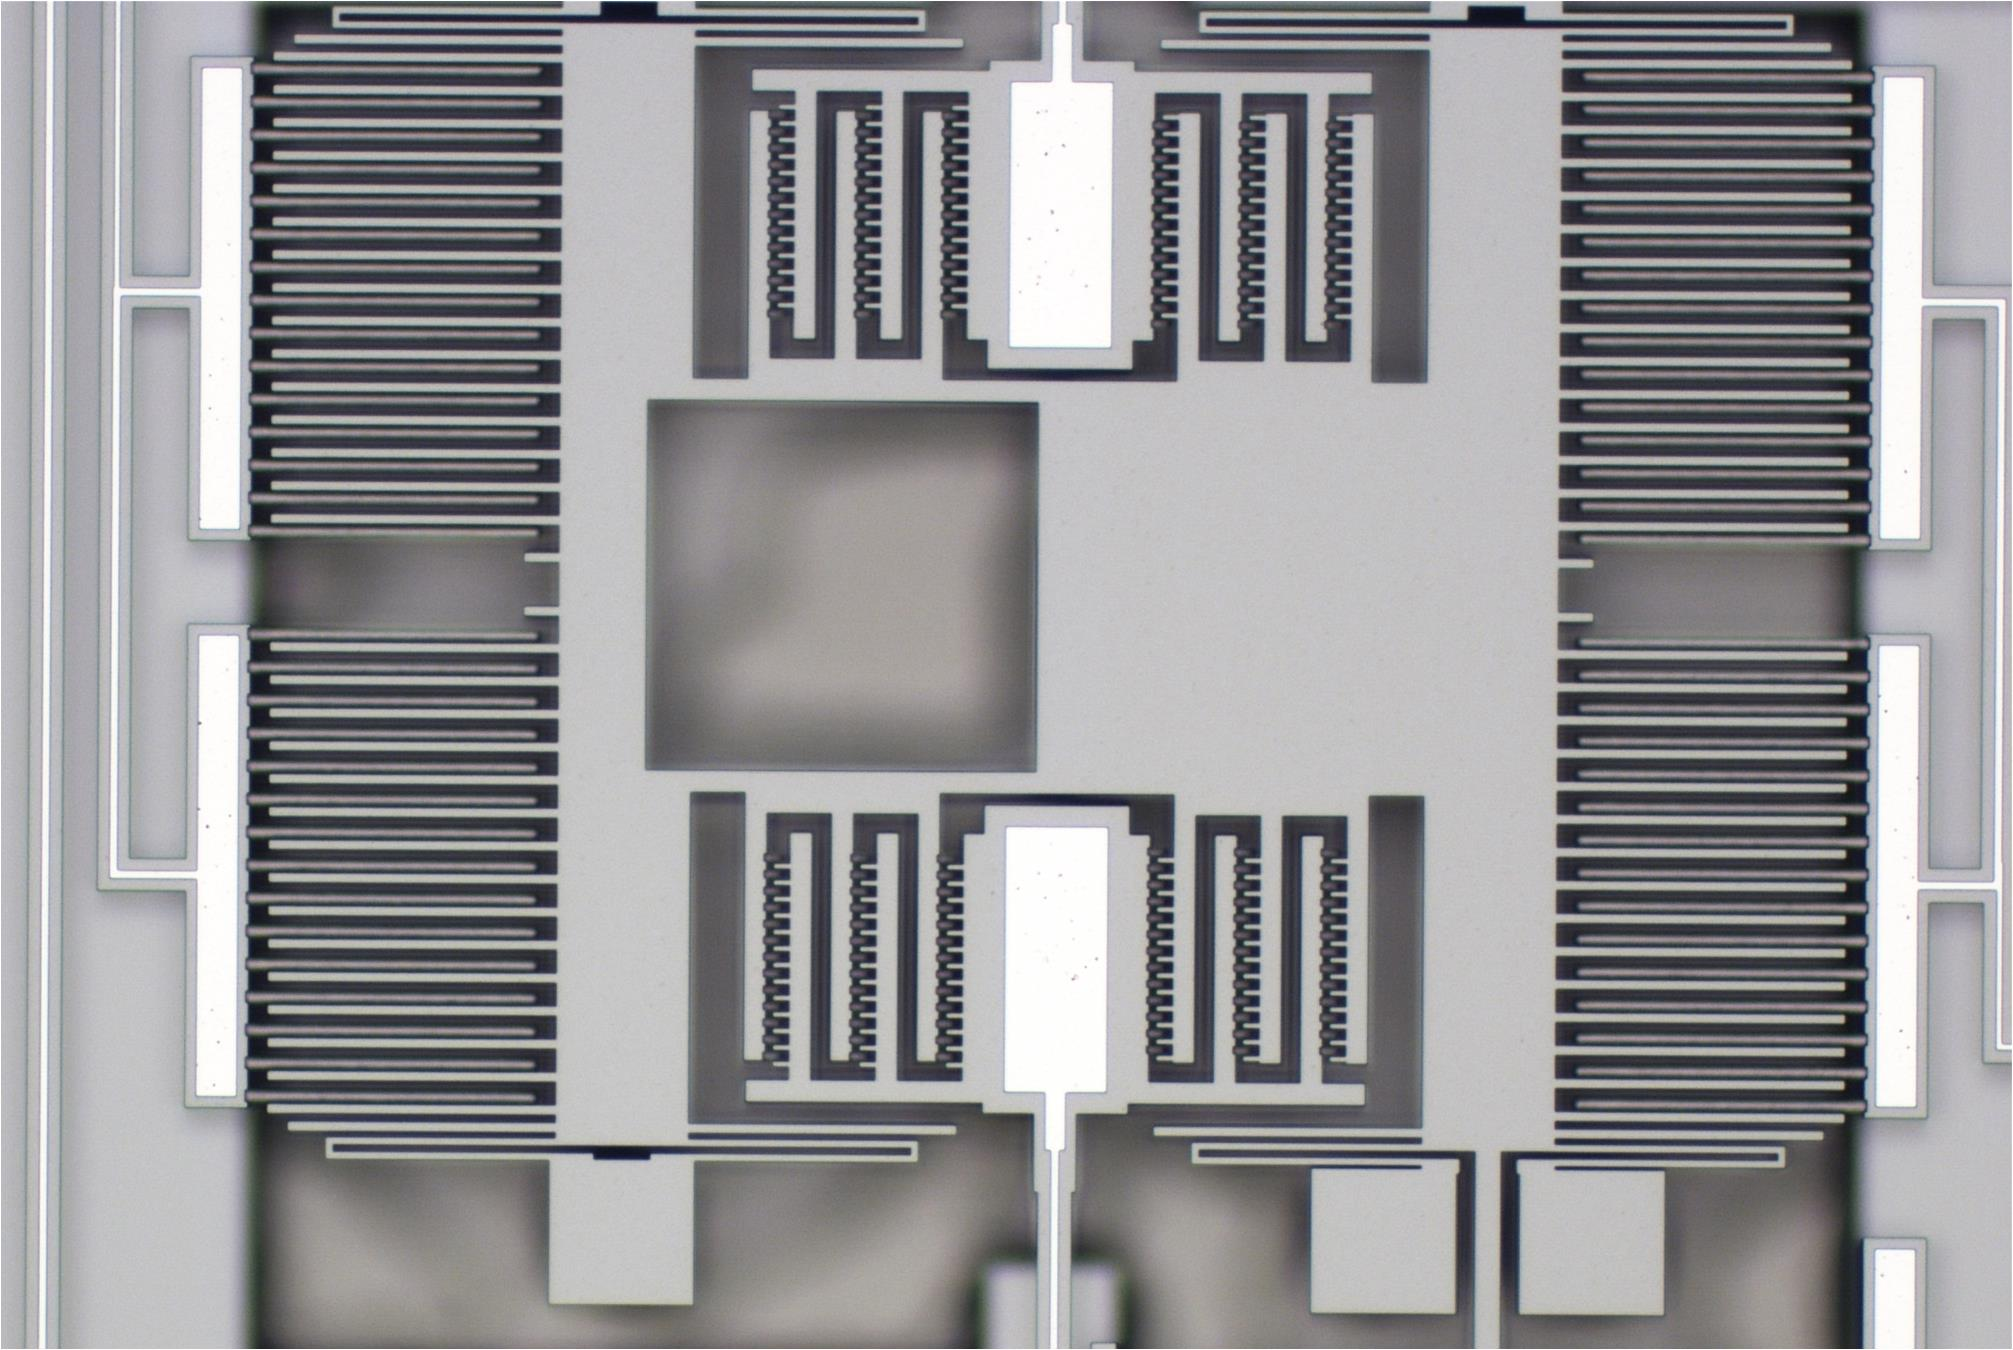
\includegraphics[height=4.5cm]{Figuras/acelerometro_mems_microscopia.png}
		\caption{Microscopia de um acelerômetro MEMS capacitivo \cite{europractice_accel}.}
	\end{subfigure}
	\hfill
	\begin{subfigure}[b]{0.4\textwidth}
		\centering
		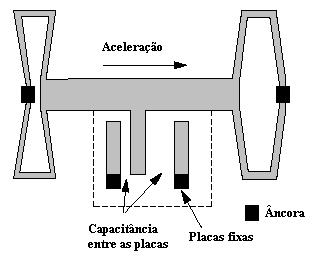
\includegraphics[height=4.5cm]{Figuras/acelerometro_esquema.png}
		\caption{Esquema simplificado do acelerômetro capacitivo \cite{ufpr_accel}.}
	\end{subfigure}
	\caption{Estrutura interna de um acelerômetro MEMS capacitivo.}
	\label{fig:mems}
\end{figure}

\subsection{Tipos de Acelerômetros}
Existem diferentes tipos de acelerômetros, que se diferenciam pela forma como o deslocamento da massa é convertido em sinal elétrico. Nos piezoelétricos, a massa pressiona um cristal que gera carga elétrica proporcional à força, eles respondem bem a variações rápidas, mas não conseguem medir acelerações constantes, como a da gravidade \cite[pp.~187--189]{aguirre2013fundamentos}. Nos piezorresistivos, a deformação das molas altera a resistência de extensômetros ligados a elas. Já nos capacitivos, que é o caso do MPU 6050, o deslocamento altera a capacitância entre as placas, como descrito na seção anterior. Esse tipo consegue medir aceleração estática, como a da gravidade, o que é verificado na Seção~\ref{sec:verificacao}.

\subsection{Erros e Fontes de Incerteza}

Os erros nas medições de um acelerômetro MEMS podem decorrer de \textit{offset}, resolução limitada e desalinhamento em relação ao sistema de coordenadas de referência. Em movimentos de rotação, a distância entre o sensor e o centro de rotação também pode introduzir erros associados à aceleração angular. Esses fatores reduzem a precisão das medições e devem ser considerados na calibração \cite{ghanipoor2020}.

\subsection{Acelerômetro do MPU 6050}
O MPU 6050 possui em um mesmo chip um acelerômetro e um giroscópio de três eixos. No acelerômetro, cada eixo possui a sua própria massa de prova, e o deslocamento dela é medido de forma diferencial por capacitores. Cada eixo tem um conversor analógico-digital sigma-delta de 16 bits e o fator de escala já vem calibrado de fábrica. Quando o sensor está parado sobre uma superfície plana, ele deve medir 0 g nos eixos X e Y e +1 g no eixo Z \cite{mpu6050}.

A comunicação com o sensor é feita pelo protocolo I$^2$C e a faixa de medição ($\pm 2$, $\pm 4$, $\pm 8$ ou $\pm 16$ g) é escolhida pelo registrador \texttt{ACCEL\_CONFIG}. Os valores lidos em cada eixo são convertidos para unidades de gravidade dividindo a leitura pela sensibilidade da faixa escolhida, que no caso de $\pm 2$~g é 16384~LSB/g.

\subsection{Característica do Sensor}

As características principais fornecidas pelo fabricante do sensor MPU 6050 são apresentadas na Tabela~\ref{tab:parâmetros}. A faixa de medição do sensor é de até $\pm 16\,\mathrm{g}$, com resolução a partir de $0{,}061\,\mathrm{mg/LSB}$ e sensibilidade de $16384\,\mathrm{LSB/g}$. Esses valores podem ser alterados entre 4 diferentes faixas de medição, configuradas a partir de um dos registradores do sensor. A não linearidade do sensor é de $0{,}5\%$ e o conversor analógico-digital tem resolução de 16 bits.

\begin{table}[H]
	\begin{center}
	\begin{tabular}{|c|c|c|c|c|} \hline
		\textbf{Parâmetro} & \textbf{Mínimo} & \textbf{Típico} & \textbf{Máximo} & \textbf{Unidade} \\ \hline
		Resolução do ADC & & 16 & & bits \\ \hline
		Amplitude de faixa nominal & $\pm 2$ & & $\pm 16$ & g \\ \hline
		Sensibilidade & 2048 & & 16384 & LSB/g \\ \hline
		Resolução & 0,061 & & 0,488 & mg/LSB \\ \hline
		Não linearidade & & 0,5 & & \% \\ \hline
		\textit{Offset} de zero-g (X e Y) & & $\pm 50$ & & mg \\ \hline
		\textit{Offset} de zero-g (Z) & & $\pm 80$ & & mg \\ \hline
		Sensibilidade cruzada & & $\pm 2$ & & \% \\ \hline
		Densidade de ruído & & 400 & & $\mu$g/$\sqrt{\mathrm{Hz}}$ \\ \hline
	\end{tabular}
	\caption{Parâmetros do sensor MPU 6050, extraídos do \textit{datasheet} \cite{mpu6050}.}
	\label{tab:parâmetros}
	\end{center}
\end{table}

\section{Verificação Experimental}
\label{sec:verificacao}
A Figura~\ref{fig:montagem} mostra a montagem utilizada, com o MPU 6050 ligado a um ESP32 pelo barramento I$^2$C.

\begin{figure}[H]
	\centering
	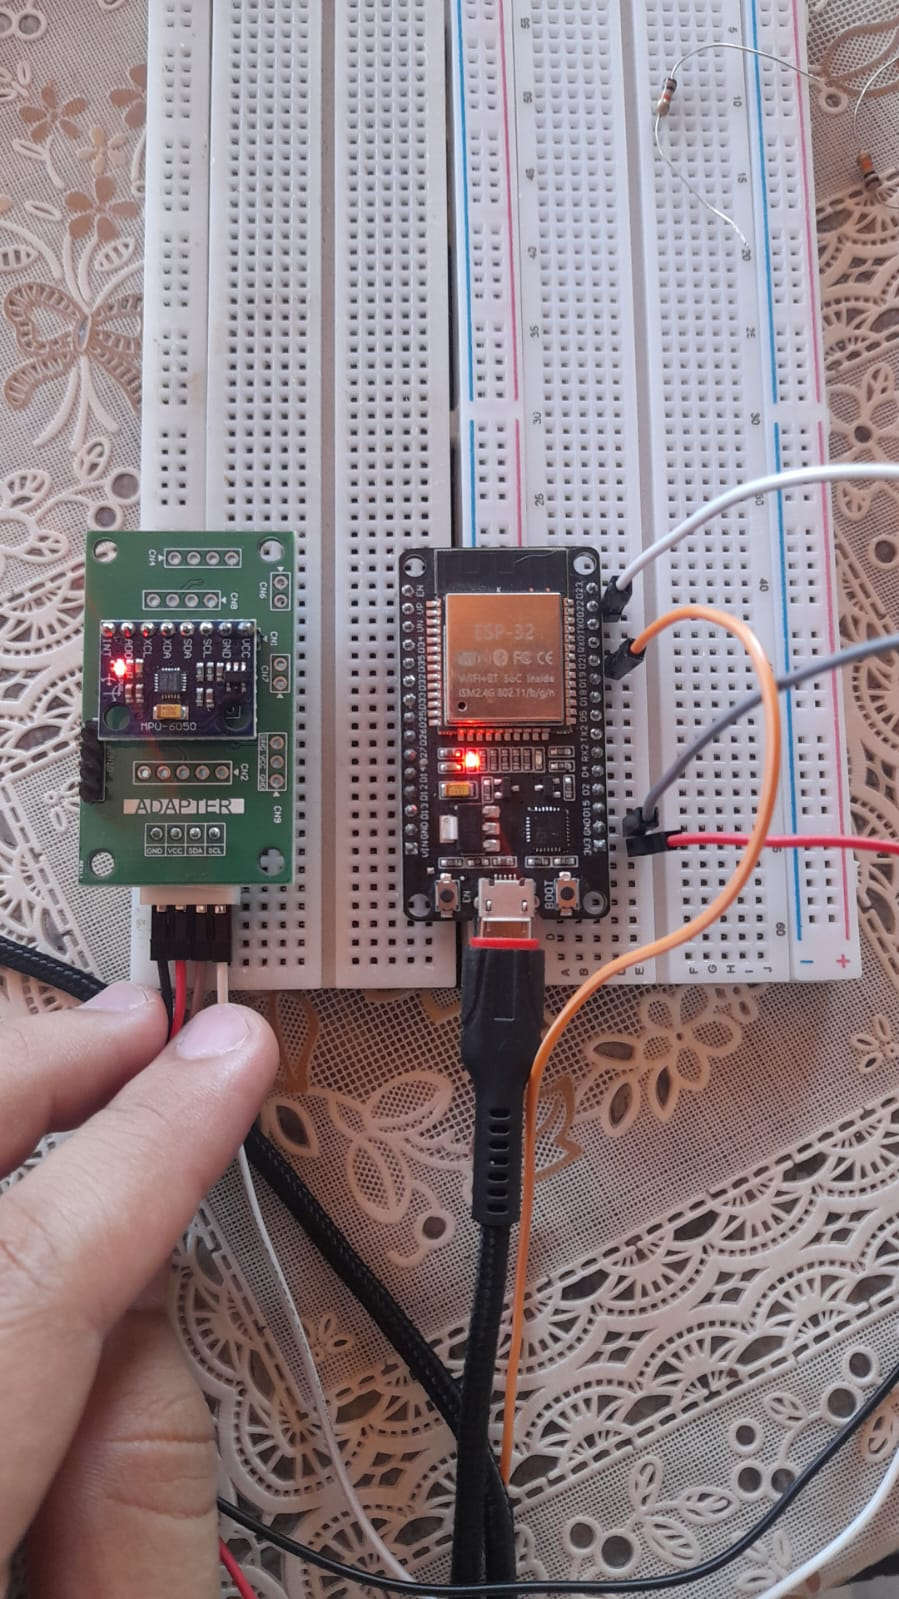
\includegraphics[width=0.4\textwidth, trim=50bp 600bp 19bp 470bp, clip]{Figuras/montagem_esp32_mpu6050.png}
	\caption{Montagem utilizada: MPU 6050 (à esquerda) ligado ao ESP32 (à direita).}
	\label{fig:montagem}
\end{figure}

O sensor foi mantido em repouso sobre a bancada em seis posições, duas para cada eixo, girando a placa para que a gravidade apontasse primeiro no sentido positivo e depois no sentido negativo do eixo em teste. Em cada posição foram registrados cerca de 10 segundos de leitura simultânea dos três eixos. A Figura~\ref{fig:verificacao_experimental} reúne os seis ensaios.

Em todos eles o eixo alinhado com a vertical fica próximo de $\pm 1\,\mathrm{g}$ e os outros dois, perto de zero, como se espera do sensor em repouso. As leituras não coincidem exatamente com esses valores: o eixo Z, por exemplo, indica cerca de $0{,}1\,\mathrm{g}$ nos ensaios em que deveria ler zero. Esse desvio soma o erro de zero do próprio sensor, informado no \textit{datasheet}, ao desalinhamento entre a placa e a horizontal, já que a superfície de apoio não está perfeitamente nivelada.

\begin{figure}[H]
	\centering
	\begin{subfigure}[t]{0.32\textwidth}
		\centering
		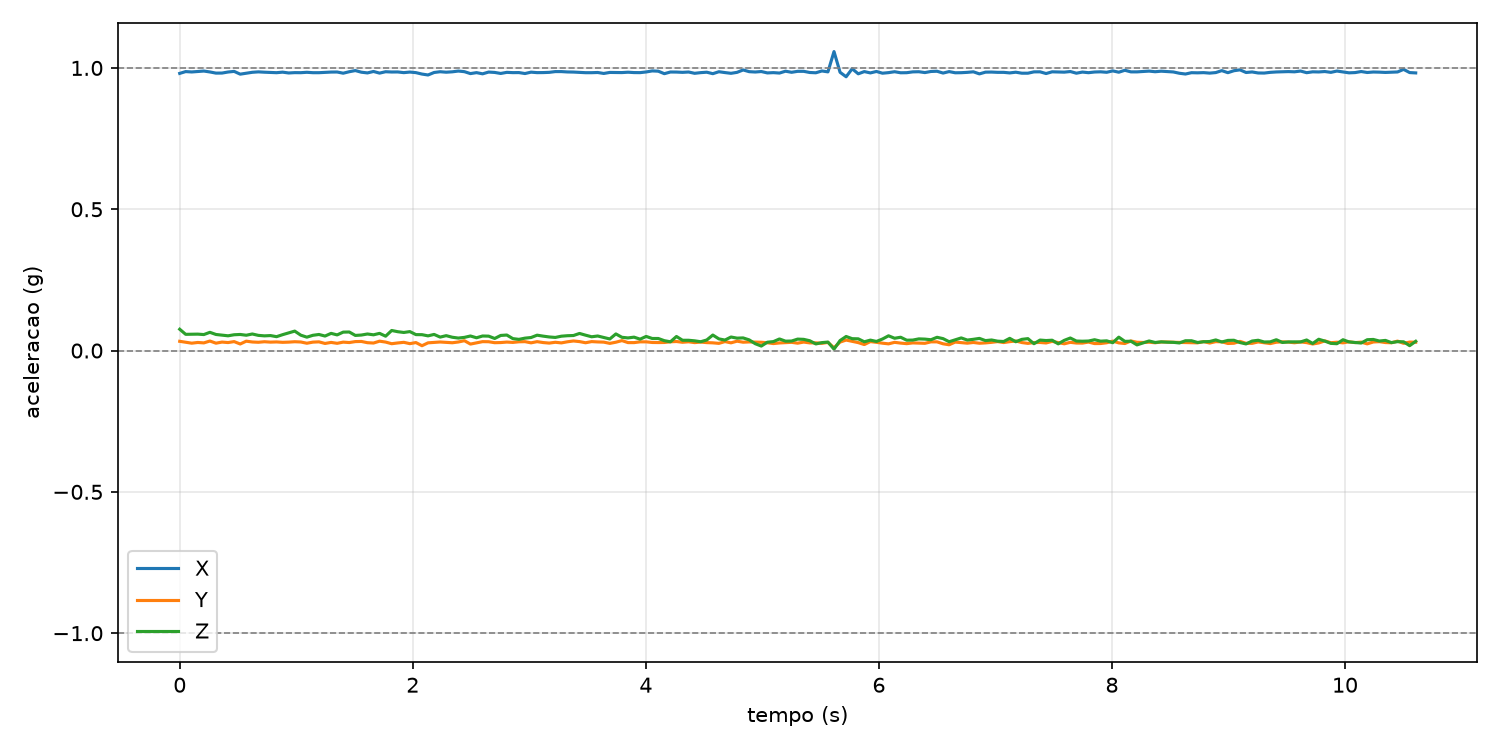
\includegraphics[width=\linewidth]{Figuras/apoiado_na_borda_X_para_baixo.png}
		\caption{Placa apoiada na borda, com o eixo X na vertical. X fica em torno de $+1\,g$.}
		\label{fig:x_positivo}
	\end{subfigure}
	\hfill
	\begin{subfigure}[t]{0.32\textwidth}
		\centering
		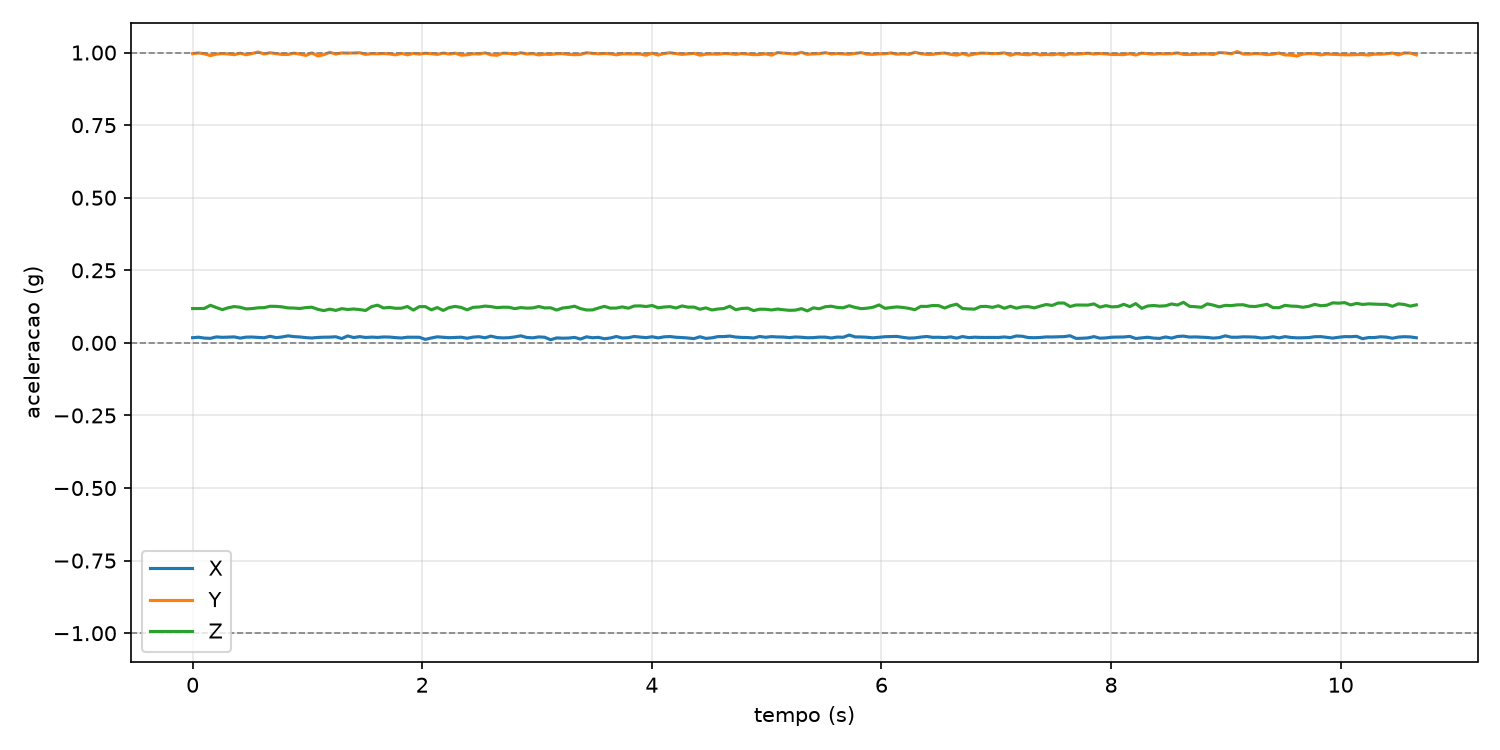
\includegraphics[width=\linewidth]{Figuras/apoiado_na_borda_Y_para_baixo.png}
		\caption{Placa apoiada na borda com o eixo Y na vertical, lendo perto de $+1\,g$.}
		\label{fig:y_positivo}
	\end{subfigure}
	\hfill
	\begin{subfigure}[t]{0.32\textwidth}
		\centering
		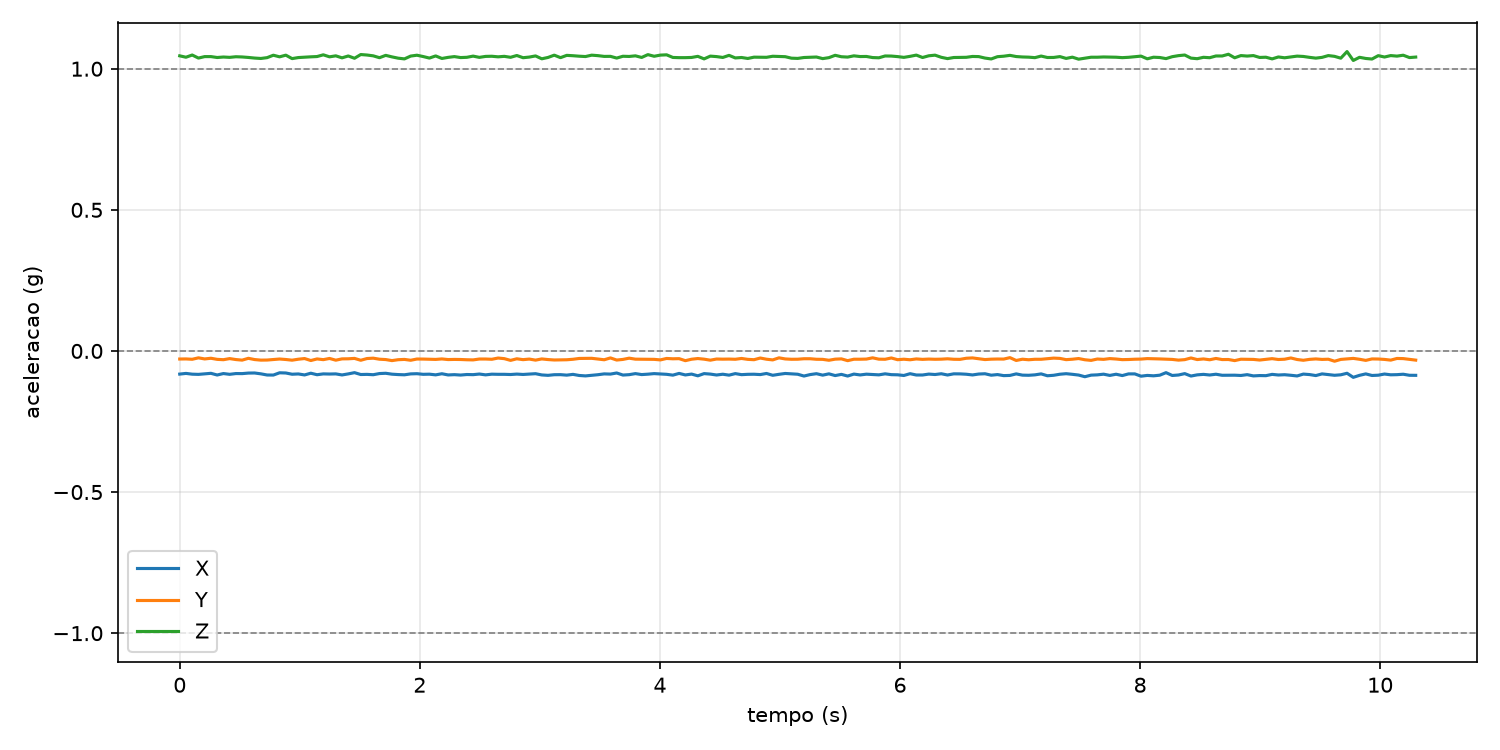
\includegraphics[width=\linewidth]{Figuras/deitado_componentes_para_cima_Z.png}
		\caption{Placa deitada, componentes voltados para cima. Z marca pouco mais de $+1\,g$.}
		\label{fig:z_positivo}
	\end{subfigure}

	\vspace{0.2cm}

	\begin{subfigure}[t]{0.32\textwidth}
		\centering
		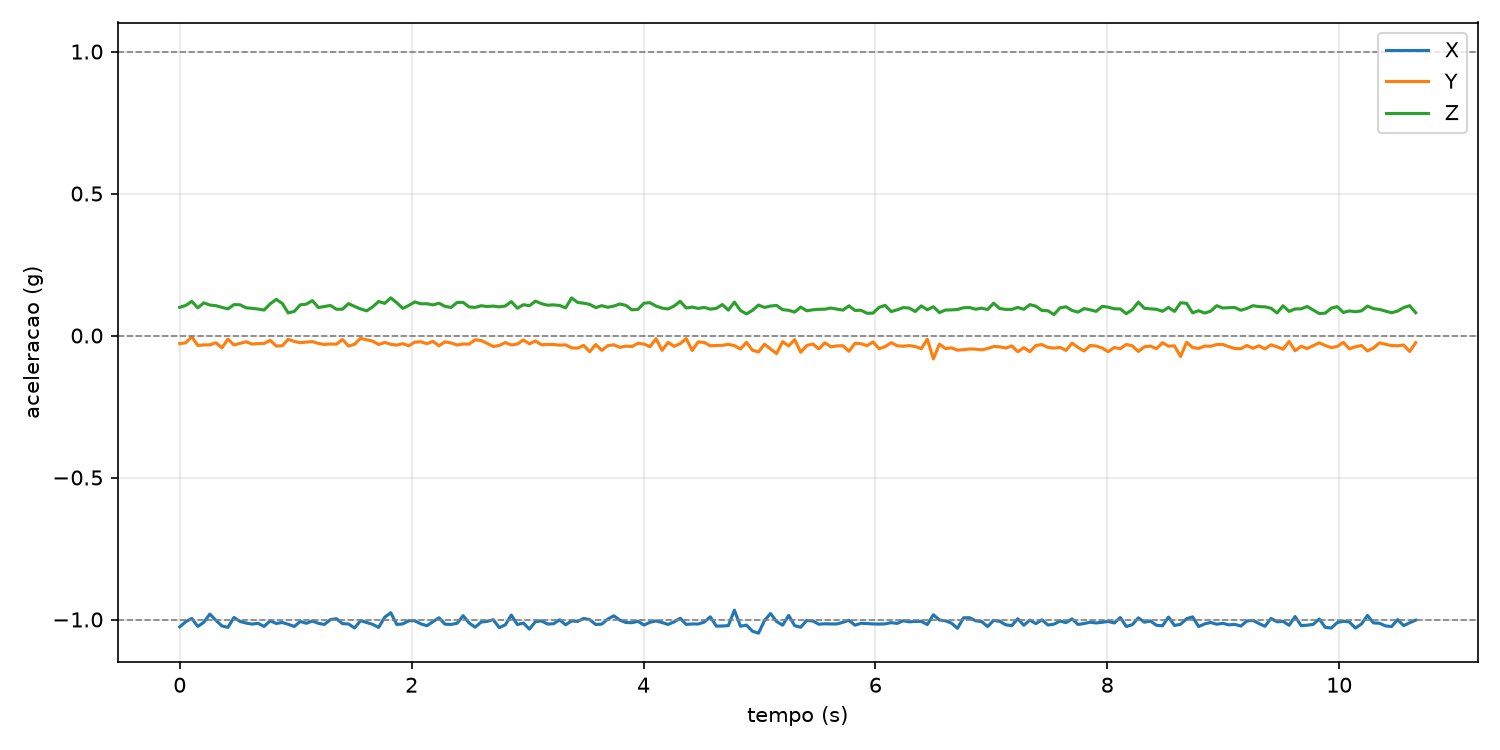
\includegraphics[width=\linewidth]{Figuras/borda_oposta_X_para_cima.png}
		\caption{A mesma placa virada para a borda oposta. O eixo X passa a marcar cerca de $-1\,g$.}
		\label{fig:x_negativo}
	\end{subfigure}
	\hfill
	\begin{subfigure}[t]{0.32\textwidth}
		\centering
		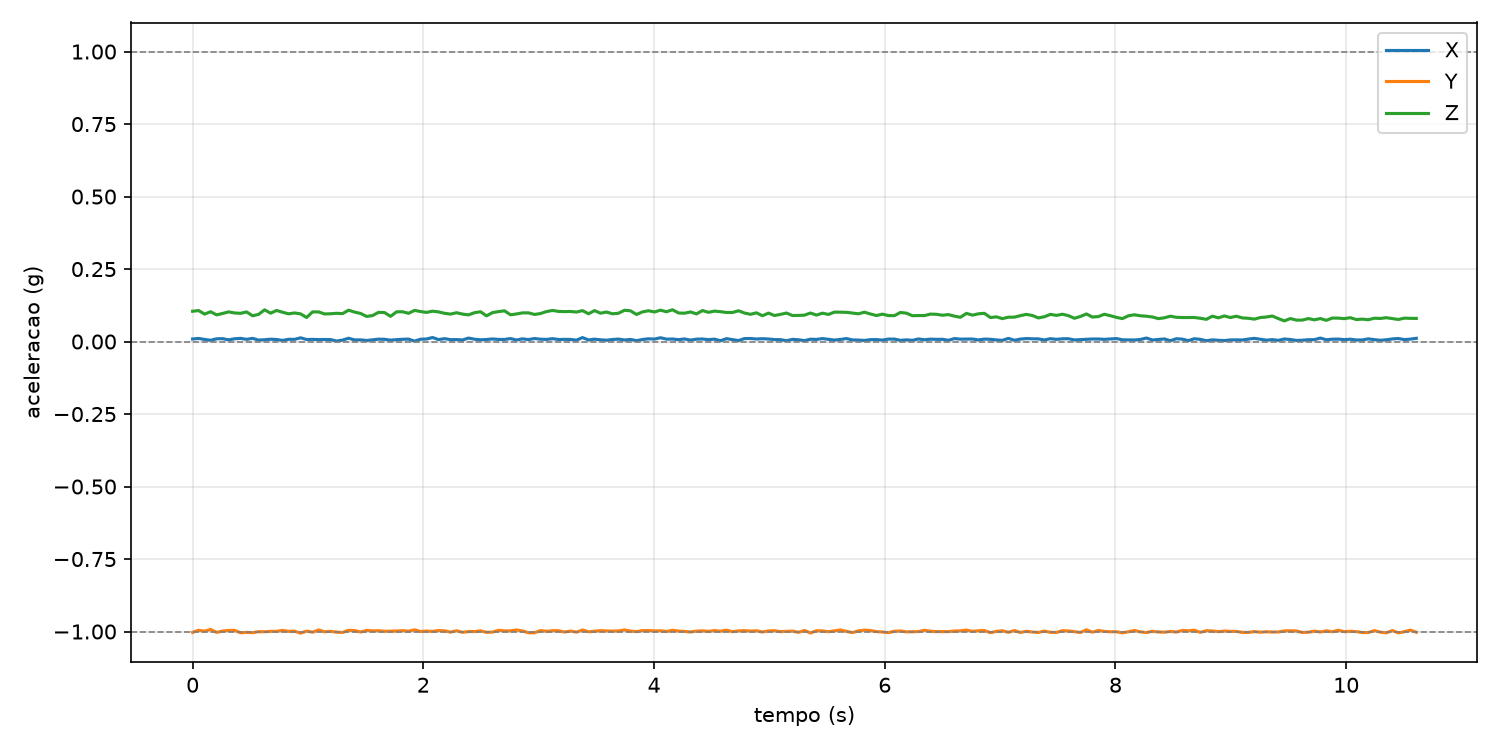
\includegraphics[width=\linewidth]{Figuras/borda_oposta_Y_para_cima.png}
		\caption{Borda oposta, eixo Y invertido: a leitura cai para cerca de $-1\,g$.}
		\label{fig:y_negativo}
	\end{subfigure}
	\hfill
	\begin{subfigure}[t]{0.32\textwidth}
		\centering
		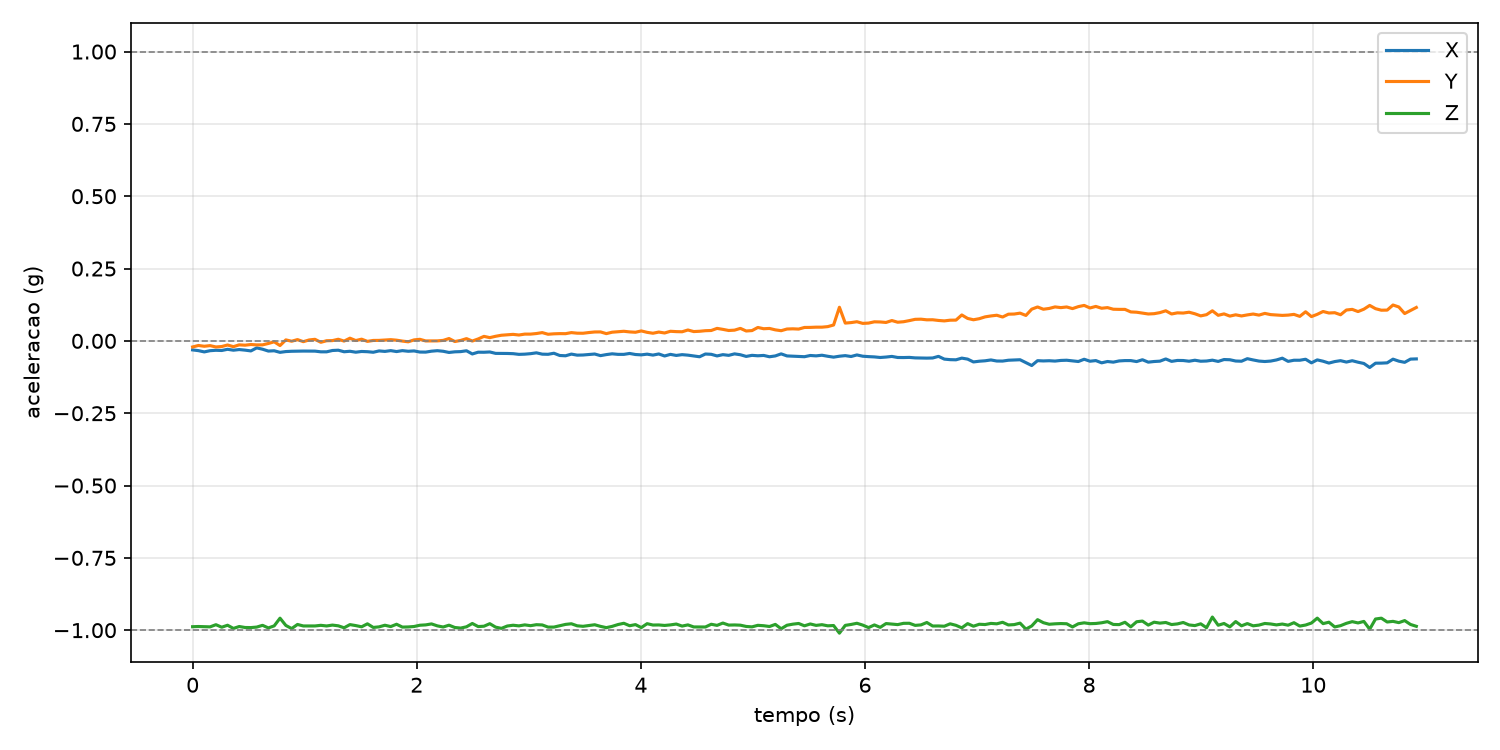
\includegraphics[width=\linewidth]{Figuras/deitado_de_cabeca_para_baixo_Z.png}
		\caption{Placa deitada de cabeça para baixo, com Z em torno de $-1\,g$.}
		\label{fig:z_negativo}
	\end{subfigure}

	\caption{Aceleração medida nos três eixos do MPU 6050 com o sensor parado, nas seis posições de ensaio, na ordem dos eixos X, Y e Z.}
	\label{fig:verificacao_experimental}
\end{figure}

\addcontentsline{toc}{section}{Referências}
\bibliographystyle{ieeetr}
\bibliography{referencias}

\end{document}
